\chapter{Inbetriebnahme}
\label{cha:Inbetriebnahme}

Die Entwicklung der Regelsoftware und die Inbetriebnahme der Kälteanlage gestaltet sich als ein kleinschrittiger, iterativer Prozess. 

\section{Elektrische Inbetriebnahme}
\label{Inbetriebnahme_ACDC}

Die elektrische Inbetriebnahme der elektrischen Steuerung der Kältemaschine erfolgt durch die Kältefachfirma noch im manuellen Betrieb ohne die SPS. Die Steuerung/Regelung kann nun Schritt für Schritt auf die SPS umgelegt werden.

Zusätzlich werden die RS485-Netzwerke mit Knotenpunkten, Abschlusswiderständen, \textit{Pull-up} and \textit{Pull-Down} installiert. Alle Stecker für die Drucksensoren müssen, entsprechend des Handbuches, mit den Stichleitungen verlötet werden. Die Stichleitungen jedes Sensors werden dann in einem Knotenpunkt an das Netzwerk angeschlossen. Ein falscher Anschluss der Datenleitung an die Spannungsversorgung der Drucksensoren kann zur Zerstörung des Sensors führen. Spannungsfreies Arbeiten ist aus diesem Grund unbedingt einzuhalten. \citep{KELLER2015}
Die Sensoren können jetzt nacheinander in das RS485-Netzwerk integriert werden. 

\section{Informationstechnische Inbetriebnahme}
\label{sec:Inbetriebnahme_IT}

Zunächst werden alle Pt100-Temperatursensoren an die SPS angeschlossen und ausgelesen. 

Danach wird das erste Modbus RTU-Netzwerk in Betrieb genommen. Wichtig hierfür ist, dass alle Sensoren in einem Netzwerk die gleichen Kommunikationseinstellungen haben. Die Drucktransmitter werden über ein \textit{Write Single Register}-Befehl adressiert. Im Auslieferungszustand hat jeder Drucktransmitter die Adresse "1". Nachdem die neue Adresse in das Adressregister geschrieben worden ist, muss der Drucktransmitter neu gestartet werden. Jetzt kann er unter der neuen Adresse Befehle empfangen. 
Die Drucktransmitter werden nach einander adressiert und in das Netzwerk integriert. 

Die Expansionsventile und der Massenstromsensor werden manuell über ihr Bediendisplay eingestellt. Dann werden  auch sie in das Netzwerk integriert. 
 
Durch System Manager, der in TwinCAT 3 integriert ist,   können die Busklemmen manuell gesteuert werden. Diese Funktion wird genutzt, um die ausgegebene Klemmenspannung bzw. -strom zu prüfen, als auch den korrekten Betrieb der übrigen Komponenten zu prüfen. Nach korrekter Signalverarbeitung über den System Manager kann die Komponente an die SPS angeschlossen werden. Dann wird getestet, ob die Funktionen in dem Programm-Code korrekt das Prozessabbild an die Ausgangsklemme gegeben wird. 

Die Implementierung des Anlagenschutzes folgt. Alle softwareseitigen Schutzfunktionen, die zur Sicherheit der Anlage und des Personals dienen und aus der Risikoanalyse hervorgegangen sind, werden getestet. 

Die Regelung der Kälteanlage kann in Betrieb genommen werden. Die Reihenfolge der Inbetriebnahme der Stellsignale ist folgende:

\begin{itemize}
\item Anschluss der Heizelemente an die SPS 
\item Anschluss des Drehzahlreglers des Verflüssigungsventilators an die SPS 
\item Anschluss der Schützschalter an die SPS zur Spannungsfreigabe des Kompressor, des Ver-flüssigungs-, des Verdampfer- und des Abtauverdampferventilator, Schaltung der Magnetventile und des Vierwegeventils
\item Überspielung der Kompressor-Software mit Software für ein externes 4\dots 20 mA-Stellsignal. Dann folgt der Anschluss an die SPS und manuelle Tests per System Manager
\end{itemize}

Bei der Regelung-Inbetriebnahme wurden zunächst die nativen Grenzen für den PID-Regler begrenzt und in kleinen Schritten vergrößert. Bei der Kompressor-Regelung wurde z. B. zunächst das höchste Stellsignal auf 8 mA festgelegt und dann in 2 mA-Schritten bis 20 mA erhöht und zusätzlich die höchste Frequenz auf 50 Hz begrenzt. Erst nach der kältetechnischen Inbetriebnahme (siehe \ref{cha:Inbetriebnahme}))  wurde die Frequenz auf die maximalen 70 Hz erhöht. 

Dieses Vorgehen wurde auch beim PID-Regler für den Verflüssigungsventilator angewandt.

Die Benutzeroberfläche der Kälteanlage wird zum Schluss in Betrieb genommen, angepasst und optimiert. 

\section{Fehlersuche}
\label{sec:Fehlersuche}

Nach der gesamten Inbetriebnahme werden der stationäre Kühlbetrieb und  die Funktionalität der Abtaumethoden getestet. Weist das Anlagenverhalten Unregelmäßigkeiten auf, so muss eine Fehlersuche vorgenommen werden. Zunächst wird der mögliche Fehler in dem Programm-Code gesucht, dann auf der elektrischen Ebene und zum Schluss auf der hydraulischen Ebene. Eine Fehlerbehebung auf informationstechnischer Ebene ist meist schnell durchgeführt und ein möglicher Fehler durch Code-Anpassung behoben. 
Im Folgenden werden die Ursachen und die Behebung der folgenden Probleme erläutert:

\begin{itemize}
\item	Ungewollte Kältemittelbewegung im Anlagenstillstand und Kühlbetrieb
\item	Kälteleistungsminderung durch Kältemittelmangel und \textit{Flashgas}
\item 	Schwingender Regelkreislauf
\end{itemize}

\subsection*{Ungewollte Kältemittelbewegung im Anlagenstillstand und Kühlbetrieb}

Vor einem Anlagenstillstand wird ein Pumpdown (siehe \ref{subsec:Statusmaschine}) durchgeführt. Das schützt den Kompressor beim Wiederanlaufen vor einer starken Unterkühlung und möglichen Tropfenschlägen am Kompressoreingang. Im Sammler ist der Großteil des Kältemittels gelagert und verlässt diesen im Normalfall erst wieder im Betriebsfall. In der aktuellen Anlagenkonfiguration wird das Entweichen des flüssigen Kältemittels durch zwei Rückschlagventile und die zwei Expansionsventile sichergestellt, dargestellt in Abbildung \ref{fig:Problem1}. Es wurde festgestellt, dass die Expansionsventile nicht für diese Funktion geeignet sind. Über einen Stillstand von 12 h findet ein Druckausgleich in der ganzen Anlage statt und das Kältemittel verteilt sich im ganzen Kreislauf.

Das Problem wird kurzfristig durch das manuelle Schließen der Absperrventile nach dem Massenstromsensor im Anlagenstillstand behoben. Für eine längerfristige Lösung sollte die Installation eines zusätzlichen Magnetventils in die Einspritzleitung geprüft werden. 

Neben der Kältemittelbewegung im Anlagenstillstand, wurde auch eine Kältemittelbewegung im Kühlmodus festgestellt. Läuft die Anlage im Kühlmodus, so ist nach dem Verflüssiger flüssiges Kältemittel anzutreffen. Das flüssige Kältemittel wird nun über die Druckdifferenz in den Abtauverdampfer gedrückt und sammelt sich dort. Dem Kältemittelkreislauf wird so im Kühlbetrieb Kältemittel entzogen. Der Sammler ist nicht mehr gefüllt und es kann zu Massenstromschwankungen kommen, die wiederum in Kälteleistungsschwankungen münden. 
 Auch hier könnte die zusätzliche Installation von Magnetventilen Abhilfe schaffen. Weitere Lösungs- und Optimierungvorschläge sind in Abschnitt \ref{cha:Ausblick} zusammengetragen.  


\begin{figure}[htb]
\centering	
	\includegraphics[page=1,width=1.150\textwidth]{Pictures/Inbetriebnahme/Probleme.pdf}
\caption{Kältemittelbewegungen im Anlagenstilland (gelb markierte Ventile). Kältemittelbewegung im Kühlbetrieb in Richtung Abtauverdampfer (grün markierte Ventile). In blau hinterlegte Magnetventile sind mögliche Lösungensvorschläge zur Problembehebung.}
\label{fig:Problem1}
\end{figure}


\subsection*{Geringe Kälteleistung des Luftkühlers}

Im Kühlbetrieb im stationären Zustand sind folgende Punkte aufgefallen: 
\begin{itemize}
\item Hohe Kältemittel-Überhitzung am Ausgang des Verdampfers (20-30 K)
\item Vollständig geöffnetes Expansionsventil
\item Schnelle Vereisung der ersten Rohrlängen im Verdampfer-Wärmeübertrager
\item hoher Druckverlust zwischen Verflüssiger-Ausgang und Expansionsventil-Eingang
\item geringer Massenstrom (20-30 g/s)
\end{itemize}

Mögliche Gründe für dieses abnormale Anlagenverhalten waren :

\begin{itemize}
\item Kältemittelmangel
\item falsch dimensioniertes Expansionsventil
\item \textit{Flash-Gas} vor dem Expansionsventil
\end{itemize}

Zunächst werden 6 kg zusätzliches Kältemittel nachgefüllt. Die gesamte Kältemittelmenge liegt jetzt bei insgesamt 20 kg. Nach einer Überschlagung der Druckverluste zwischen Expansionsventil und Verflüssiger, kann der Druckverlust als deutlich zu hoch eingestuft werden. Kondensiertes Wasser auf den Rohrleitungen nach dem Trockner, sowie Bläschen im Schauglas weisen auf \textit{Flash-Gas} hin, vgl. \citep{GAGKG2010}.
Durch einen zu hohen Druckverlust kommt es zur Verdampfung des Kältemittels bevor es durch das Expansionsventil entspannt wird. Durch die Gasbläschen erhöht sich das spezifische Kältemittel-Volumen und verringern gleichzeitig den Massenstrom durch das Expansionsventil. Das Expansionsventil versucht die Überhitzung zu senken, indem es sich öffnet. In diesem Fall versucht das Expansionsventil durch eine vollständige Öffnung einen höheren Massenstrom zu erwirken. Abbildung \ref{fig:Problem_Trockner} zeigt die Zustandspunkte der Anlage im log p,h-Diagramm. Im Diagramm sind der hohe Druckverlust und die hohe Überhitzung mit gelben Pfeilen gekennzeichnet. 

Das Problem konnte durch das Austauschen des Trockners behoben werden. Der Druckverlust zwischen Expansionsventil und Verflüssiger-Austritt verringerte sich von knappen 3 auf 0,5 bar. Das Expansionsventil regelte nun mit einer Öffnung von 50-55 $\%$ auf die vorgegebene Überhitzung von 6 K. 


\begin{figure}[h]
\centering		\includegraphics[page= 2,width=1.120\textwidth]{Pictures/Inbetriebnahme/Inbetriebnahme_Probleme.pdf}
\caption{Hohe Kältemittel-Überhitzung nach Verdampfer und hoher Druckverlust zwischen Expansionsventil und Verflüssiger dargestellt im log p,h-Diagramm}
\label{fig:Problem_Trockner}
\end{figure}

\begin{figure}[h]
\centering		\includegraphics[page= 36,width=1.05\textwidth]{Pictures/Inbetriebnahme/Inbetriebnahme_Probleme.pdf}
\caption{Zustandspunkte der Kältemaschine nach Fehlerbehebung im log p, h-Diagramm}
\label{fig:KA_OK}
\end{figure}

\newpage
\subsection*{Schwingender Regelkreislauf}

Da die Expansionsventile nur durch den Modbus RTU ausgelesen werden und nicht gesteuert, können sie nur mir einer PID-Parametereinstellung betrieben werden. Mit den Auslieferungsparameter für den \textsc{Carel}-PID-Regler wurde im Kühlbetrieb eine Schwingung um den Sollwert der Überhitzung ($\pm$ 4 K) festgestellt. 

Der Grund hierfür ist der örtliche Abstand zwischen Verdampfer-Ausgang und Position des Druck- und Temperaturfühlers vom Expansionsventil (ca. 3 m). Der Temperaturfühler ist, wie in der Praxis üblich, nur ein Oberflächensensor. Der Temperaturfühler erfasst die Temperaturänderung, ausgelöst durch eine Ventilöffnungsänderung,  erst mit einer Verzögerung von 90-120 s. Ein anderes Pt100-Element (\textit{Temp$\_$VD$\_$out}), angebracht unmittelbar am Verdampfer-Ausgang,  misst eine Temperaturänderung nach einer Ventilöffnungsänderung bereits nach 10-15 s. 

Eine kurzfristige Lösung des Problems ist die Veränderung der Regelparameter des Expansionsventils nach dem Einschwingvorgang bzw. Herunterkühlen der Klimakammer (t $\approx$ 20 min). Um einen schwingenden Regelkreis im stationären Zustand zu vermeiden, wurden die Parameter manuell umgestellt. 

\begin{table}[htb]
\centering
\caption{Werte für \textsc{Carel}-PID-Regler für Einschwingvorgang und stationären Betrieb}\vspace{6pt}
\begin{tabular}{lll}
\hline 
\textbf{PID-Parameter} & \textbf{Einschwingvorgang} & \textbf{Stationärer Betrieb} \\ 
\hline 
\hline
KP & 15 & 5 \\ 
\hline 
Integralzeit & 150 ms & 490 ms \\ 
\hline 
Differentialzeit & 5 s & 5 s \\ 
\hline 
\hline
\end{tabular} 
\label{tab:Regler_Uebersicht}
\end{table}

%\section{Kalibrierung Wägesystem}
%\label{sec:Waegesystem}

%Wie schon im Abschnitt \ref{sec:Waegesystem} erwähnt worden ist, muss das Wägesystem vor jeder Messung kalibriert werden. Für die Kalibierung sind folgende Schritte notwendig:

%\begin{itemize}
%\item Waagen mit 2 kg vorbelasten
%\item Gewichtskalibrierung mit in 500 g Schritten von 500 g bis 2500 g. %(Anleitung ist in der GUI implementiert)
%\item Ventilatorkalibrierung
%\end{itemize}



\section{Versuche}
\label{sec:Versuche}

Nach der Inbetriebnahme und Behebung der aufgelisteten Defizite werden erste Vereisungs- und Abtauversuche durchgeführt. Der Luftkühler befindet sich in der Klimakammer, die auf 2 °C und \mbox{90 $\%$} Luftfeuchtigkeit eingestellt ist und somit als Wärmequelle dient. Nachdem der Luftkühler 1 h vereist worden ist, wird er wieder abgetaut. Die Abtaumethode wird hierbei variiert. Die Ergebnisse für die Vereisungs- und Abtauphase werden im Folgenden dargestellt und diskutiert. In Tabelle \ref{tab:Versuchsreihe} sind die drei Versuchsreihen mit den dazugehörigen Vereisungszeiten und gewählten Abtaumethoden zu finden. 


\begin{table}[htb]
\centering
\caption{Versuchsreihen}\vspace{6pt}
\begin{tabular}{llll}
\hline 
\textbf{Versuchsreihe} & \textbf{Vereisungszeit} & \textbf{Abtaumethode} & \textbf{Position der vier Oberflächen-Pt100} \\ 
\hline 
\hline 
I & 47 min  & Heißgas-Oben & Stack-Eingang \\ 
\hline 
II & 53 min  & Heißgas-Oben & Verteilt über unterstes Stack \\ 
\hline 
III & 59 min & Elektrisch & Stack-Eingang \\ 
\hline 
\hline 
\end{tabular} 
\label{tab:Versuchsreihe}
\end{table}


\subsubsection*{Versuchsreihe I: Vereisen}


In den nachfolgenden Diagrammen sind die Temperatur- und Druckverläufe am Luftkühler dargestellt. Das Diagramm \ref{fig:VereisenI} stellt die Verläufe für die Versuchsreihe I dar. Die Druckverläufe von Ein- und Ausgang zeigen einen schwingenden Verlauf mit der Periodendauer der gesamten Vereisungszeit. Der Druck am Eingang beträgt durchschnittlich 3,7 bar, am Ausgang durchschnittlich 2,2 bar. Der Druckabfall über den Venturiverteiler und Wärmeübertrager beträgt konstante 1,5 bar über die Vereisungszeit. 

Die Temperaturverläufe sind am Eingang und an den Oberflächensensoren weitgehend konstant und führen wie die Druckverläufe eine Schwingung mit der Periodendauer von ca. 2200 s durch. Am Eingang schwankt die Temperatur in dieser Zeit zwischen 5,9 °C und 7,8 °C. Im Durchschnitt liegt sie bei 7,1 °C. Die Oberflächensensoren betragen im Durchschnitt - 6 °C. Auffällig ist die Temperaturspreizung zwischen den Oberflächensensoren. Zwischen dem Eingang des obersten Einspritzungsrohrs (\textit{TEMP$\_$VD$\_$surface$\_$6}) und dem untersten Einspritzungsrohr (\textit{TEMP$\_$VD$\_$surface$\_$2}) beträgt die Temperaturdiffernez zu jedem Zeitpunkt ca. 1 K. 

Die Eingangstemperatur, die noch vor dem Venturiverteiler gemessen wird, verzeichnet in einem kurzen Zeitraum starke periodische Schwankungen um mehrere Kelvin. Die Schwankungen werden durch die Expansionsventilöffnungsänderung ausgelöst, sprich die Überhitzungsregelung.  Die Schwankungen gilt es zu vermeiden und werden im Abschnitt \textit{Expansionsventil: PID-Parameter-Vergleich} näher diskutiert. 

\begin{figure}[htb]
\centering		\includegraphics[page=1,width=1.08\textwidth]{Pictures/Inbetriebnahme/Abtaumethoden_Tempverlaufe_Vereisen.pdf}
\caption{Versuchsreihe I: Temperaturverläufe am Luftkühler (VD) während Vereisungszeit}
\label{fig:VereisenI}
\end{figure}


\subsubsection*{Versuchsreihe II: Vereisen}

Die Versuchsreihe II zeigt im Vergleich zur Versuchsreihe I unterschiedliche Temperatur- und Druckverläufe. Der Druckverlauf am Ein- und Ausgang zeigt einen instationären Verlauf bis zur Zeit von 2200 s. Danach ist ein stationärer Zustand erreicht. Im stationären Zustand werden Druckwerte wie in der Versuchsreihe I erreicht. Der instationäre Verlauf spiegelt sich auch in den Temperaturverläufen wider. Die Instationärität wird hervorgerufen durch ein sehr langsam schließendes Expansionsventil. Der Regler der Überhitzungsregelung ist in dieser Versuchsreihe deutlich träger eingestellt als noch bei der Versuchsreihe I. 

Ab 750 s sind sprunghafte Temperaturänderungen an den Oberflächensensoren zu erkennen. Mögliche Ursachen hierfür sind die einsetzende Abtauung der Klimakammer und/oder Türöffnungen während des Versuchs.  Bei zukünftigen Versuchen gilt dies zu vermeiden. Zum Ende der Vereisungsphase, im stationären Zustand, treten am Verdampfereingang erneut periodische Temperaturschwankungen auf. 

\begin{figure}[htb]
\centering		\includegraphics[page=2,width=1.08\textwidth]{Pictures/Inbetriebnahme/Abtaumethoden_Tempverlaufe_Vereisen.pdf}
\caption{Versuchsreihe II: Temperaturverläufe am Luftkühler (VD) während Vereisungszeit}
\label{fig:VereisenII}
\end{figure}


\subsubsection*{Versuchsreihe III: Vereisen}

Die Versuchsreihe III zeigt, wie schon Versuchsreihe II, zunächst einen instationären und später, ab 1800 s, einen stationären Verlauf. Erneut ist ein träg eingestellter PID-Regler für die Überhitzungsregelung der Grund für dieses Verhalten. Die Oberflächensensoren messen im Durchschnitt -5,5 °C. Die Eingangs- und Ausgangstemperatur liegen im Durchschnitt für die stationäre Phase bei 7 °C und -3,5 °C. Der Druck am Eingang beträgt im Durchschnitt 3,7 bar und der Ausgangsdruck liegt im Durchschnitt 2,2 bar.  


\begin{figure}[htb]
\centering		\includegraphics[page=3,width=1.08\textwidth]{Pictures/Inbetriebnahme/Abtaumethoden_Tempverlaufe_Vereisen.pdf}
\caption{Versuchsreihe III: Temperaturverläufe am Luftkühler (VD) während Vereisungszeit}
\label{fig:VereisenIII}
\end{figure}


\newpage
\subsubsection*{Versuchsreihe I: Abtauen mittels \textit{Heißgas-Oben}}

Das Diagramm \ref{fig:I_Heissgas_oben}(a) zeigt den Verlauf der Temperatursensoren am Luftkühler über die Abtauzeit. Zu Beginn des Abtauens wird ein Pumpdown durchgeführt. Dann wird das Vierwegeventil geschaltet, der Kompressor läuft an und heißes Gas beginnt durch den Verdampfer zu strömen. Alle Temperaturen steigen in der Abtauzeit von 2 min simultan an. Die maximale Temperatur von 43,3 °C werden am Ende der Abtauzeit am Ein- und Ausgang des Verdampfers erreicht. 
Am Eingang der Wärmetauscherstacks werden maximal 34,8 °C erlangt. Am obersten Stackeingang (\textit{Temp$\_$VD$\_$surface6}) werden nur 29,5 °C erreicht. 

Nach der Abtauzeit folgt die Abtropfzeit von 10 min. Alle Temperaturen fallen über diesen Zeitraum. Die höchste Temperatur ist am Eingang des Verdampfers zu verzeichnen. Die Oberflächentemperaturänderung wird kleiner und die Temperaturen streben gegen einen Grenzwert. 

\textit{Temp$\_$VD$\_$-surface6}, positioniert am obersten Wärmeübertrager-Eingang, bleibt nach 550 s bei konstanten  10,5 °C. Ein möglicher Grund hierfür ist die natürliche Konvektion innerhalb des Wärmeübertrager während der Abtropfzeit. Die abgegebene Wärme steigt nach oben und führt so zu einer Temperaturschichtung. Die unteren zwei Oberflächensensoren (\textit{Temp$\_$VD$\_$surface2}~ und  \textit{Temp$\_$VD-$\_$surface4}) messen am Ende der Abtropfzeit, bei 810 s, eine Temperatur von 2,3 °C. Zwischen dem obersten und untersten Oberflächentemperatursensor ist eine Temperaturspreizung von 8 K zu verzeichnen. 

Das Diagramm \ref{fig:I_Heissgas_oben}(b) zeigt die Massenverläufe und die Öffnung der Expansionsventils über die gesamte Abtauphase. Mit dem Pumpdown sinkt die Masse des Verdampfers, weil das noch vorhandene Kältemittel abgesaugt wird und der Verdampfer an Gewicht verliert. Mit Beginn der Abtauung durch Heißgas steigt sofort die Masse des Verdampfers. So steigt die Verdampfermase innerhalb der 2 min um ca. 3,8 kg an. Nach dem Beginn der Abtropfphase sinkt die Verdampfermasse erneut, da das Eis geschmolzen ist und nun über den Abfluss abgeführt wird. Die Abtropfmasse steigt nun stetig an und der Verdampfer wird wieder leichter. In der Abtropfphase wird der Verdampfer um 910 g leichter. Die gesamte Abtropfmasse beträgt 2456 g. 


Nach 600 s Abtropfzeit beginnt die Kälteanlage wieder mit dem Kühlmodus. Alle Temperaturen sinken und der Zyklus beginnt erneut. 



\begin{figure}%[h]
\centering
\subfigure[Temperaturverläufe am Luftkühler. Oberflächen-Temperatursensoren(\textit{surface}) sind angebracht am Einspritzrohr]
{\includegraphics[page=1,width=1.03\textwidth]{Pictures/Inbetriebnahme/Abtaumethoden_Tempverlaufe.pdf}}
\subfigure[Verläufe von der Abtropfmasse und Verdampfermasse, Öffnung des Expansionsventils aufgetragen über die Zeit]{\includegraphics[page=21,width=1.08\textwidth]{Pictures/Inbetriebnahme/Diagramme_Versuche.pdf}}
\caption{Versuchsreihe I: Abtauen mittels \textit{Heißgas-Oben}}
\label{fig:I_Heissgas_oben}
\end{figure}

\newpage
\subsubsection*{Versuchsreihe II: Abtauen mittels \textit{Heißgas-Oben}}

In der Versuchsreihe II wird erneut mittels \textit{Heißgas-Oben} abgetaut. Die Oberflächentemperatursensoren werden für diese Messung an nur einem Wärmeübertragungsrack angebracht. Die Oberflächentemperatursensoren sind Pt100-Elemente. Ein Rack besteht aus 6 x 6 Rohrleitungen, durch die das Kältemittel geführt wird. Die Oberflächensensoren sind an folgenden Rohren angebracht: 1. Rohr (Einspritzrohr, \textit{Temp$\_$VD$\_$surfaceX12}), 12. Rohr (\textit{Temp$\_$VD$\_$surfaceX12}), 25. Rohr (\textit{Temp$\_$VD- $\_$surfaceX25}) und 36.  Rohr (\textit{Temp$\_$VD$\_$surfaceX36}).

Die höchste Temperatur wird am Verdampfereingang mit 43,9 °C erreicht. Die Temperaturverläufe zeigen ähnliche Charakteristika wie die Temperaturverläufe aus der Versuchsreihe I. Nachdem das Heißgas 2 min durch den vereisten Wärmeübertrager geströmt ist, misst jeder Sensor die örtliche maximale Temperatur.  Danach fallen alle Temperaturwerte mit ähnlicher Geschwindigkeit wie sie zuvor gestiegen waren. Nach 2 min flachen die Temperaturkurven ab und sinken mit geringer Geschwindigkeit während der Abtropfphase weiter. Die Temperaturspreizung zwischen den Oberflächentemperaturen beträgt ca. 1,5 K. Die Oberflächentemperatur am 36. Rohr ist die wärmste und die anderen drei Oberflächentemperaturen sind nahezu gleich. Die Oberflächentemperatur am 12. Rohr \textit{Temp$\_$VD$\_$surfaceX12}) steigt nach Beginn der Heißgas-Abtauung, jedoch nicht so stark wie die anderen Oberflächentemperaturen. Die maximale Temperatur wird 60 s nach dem Ende des Abtauvorgangs, bei 310 s, mit 8 °C erreicht. Nach der Abtropfdauer startet der Kühlmodus und die Temperaturen fallen wieder. 

\begin{figure}[htb]
\centering		\includegraphics[page=2,width=0.95\textwidth]{Pictures/Inbetriebnahme/Abtaumethoden_Tempverlaufe.pdf}
\caption{Versuchsreihe II: Abtauen mittels \textit{Heißgas-Oben}}
\label{fig:II_Heissgas_oben}
\end{figure}

\newpage
\subsubsection*{Versuchsreihe III:  \textit{Elektrisches} Abtauen}

Nachdem der Verdampfer vereist worden ist, wird der Verdampfer mittels einer elektrischen Heizung abgetaut. Die elektrische Heizung umfasst 20 Heizstäbe, die in dem Wärmeübertrager integriert sind. Ein Heizstab hat eine maximale Leistung von 220 W. Die Bodenplatte des Luftkühlers ist mit 3 Heizstäben á 625 W ausgestattet. Die gesamte elektrische Abtauleistung beträgt 6,275 kW. Die Heizelemente sind stufenlos zwischen 0$\dots$10 V regelbar.  

In diesem Versuch wurde mit der maximalen Leistung, sprich 6,275 kW, abgetaut. Abbidlung \ref{fig:III}(a) zeigt die Temperatursensoren des Luftkühlers. 

Wie auch bei den Versuchsreihen I und II wird auch hier zunächst ein Pumpdown durchgeführt. Danach fängt die Abtauphase an und die Temperaturen steigen. Die Oberflächentemperatur von \textit{Temp$\_$VD$\_$surface2}), unterste Position,  steigt zu erst an und erreicht die maximale Temperatur von 16,8 °C nach 1180 s. Mit diesem Maximum endet die Abtauphase und die Abtropfphase von 10 min beginnt. Die Temperatur von \textit{Temp$\_$VD$\_$surface2}) sinken. 
Mit einer Zeitverzögerung von 400-500 s steigen auch die Temperaturen von \textit{Temp$\_$VD$\_$surface5}) und \textit{Temp$\_$VD$\_$surface6}).

Die natürliche Konvektion innerhalb des Wärmeübertragers führt zu einer Temperaturschichtung, die sich an den oberen drei Oberflächensensoren widerspiegelt.  

Der Druck ist am Ein- und Ausgang zu jederzeit während des Abtauvorgangs identisch. Der Druck steigt von anfänglich 1 bar auf 2,7 bar am Ende der Abtropfzeit an. Zwischen der Zeit von 150 s bis 1050 s steigt der Druck langsam an. Bei 1050 s kommt es zu einer hohen Druckveränderung. Innerhalb von 150 s steigt der Druck von 1,8 bar auf 2,7 bar und bleibt für die Rest der Abtropfzeit konstant. 

Insgesamt ist der \textit{elektrische} Abtauvorgang mit 1800 s knapp 800 s länger als die Abtauung per \textit{Heißgas}. Das Temperaturniveau ist mit maximalen 16,8 °C um 27 K kälter als bei einer \textit{Heißgas}-Abtauung. 

Das Diagramm in Abbildung \ref{fig:III}(b) sind die Verläufe der Verdampfermasse, Abtropfmasse und die Öffnung des E-Ventils über die Abtaudauer aufgetragen. Die Gewichtsänderung des Verdampfers beträgt 2640 g. Die Gewichtsänderung der Abtopfmasse ist 1660 g groß. Das Expansionsventi ist über die Abtaudauer geschlossen. 


%\begin{figure}[htb]
%\centering		\includegraphics[page=3,width=1.08\textwidth]{Pictures/%Inbetriebnahme/Abtaumethoden_Tempverlaufe.pdf}
%\caption{III: \textit{Elektrisch} Abtauen mit 6,275 kW Heizleistung}
%\label{fig:III_Elektrisch}
%end{figure}


\begin{figure}%[h]
\centering
\subfigure[Temperaturverläufe am Luftkühler. Oberflächen-Temperatursensoren(\textit{surface}) sind angebracht am Einspritzrohr]
{\includegraphics[page=3,width=1.02\textwidth]{Pictures/Inbetriebnahme/Abtaumethoden_Tempverlaufe.pdf}}
\subfigure[Verläufe von der Abtropfmasse und Verdampfermasse, Öffnung des Expansionsventils aufgetragen über die Zeit]{\includegraphics[page=1,width=1.08\textwidth]{Pictures/Inbetriebnahme/Abtaumethode_Gewichtsverlaufe_elektrisch.pdf}}
\caption{Versuchsreihe III: \textit{Elektrisch} abtauen mit 6,275 kW Heizleistung}
\label{fig:III}
\end{figure}


\newpage
\subsubsection*{Expansionsventil: PID-Parameter-Vergleich}
\label{subsubsec:EV}

Für eine hohe Reproduzierbarkeit der Versuche ist ein stationärer Zustand nötig. Ein instationäres System verringert die Aussagekraft über die späteren Versuchsergebnisse. Das Expansionsventil hat großen Einfluss auf die angestrebte Stationarität der Kälteanlage. Aus diesem Grund ist der Verlauf der Überhitzung für alle drei Versuchsreihen  über die Zeit aufgezeichnet. 

Das Expansionsventil kann entweder mit den PID-Parametern für den stationären Betrieb oder für den Einschwingvorgang programmiert sein. Regelt das Expansionsventil von Beginn an mit stationären PID-Parametern, so hat dies einen sehr langen Einschwingvorgang (siehe Kurve \textit{Stationäre PID-Parameter} im Diagramm \ref{fig:EV_Vergleich}).

Ist das Expansionsventil mit den Einschwing-PID-Parametern programmiert, wird der Sollwert schnell~erreicht, jedoch schwingt die Überhitzung periodisch um den Sollwert mit Abweichungen um $\pm 3$ K (siehe Kurve \textit{Einschwing-PID-Parameter} im Diagramm \ref{fig:EV_Vergleich}). 

Werden die PID-Parameter nach Erreichen des Sollwertes geändert, so verkürzt sich die Einschwingphase und die Schwingungsamplitude im stationären Zustand (siehe Kurve \textit{Einschwing + Stationäre PID-Parameter} im Diagramm \ref{fig:EV_Vergleich}). Für zukünftige Versuche werden im Abschnitt \ref{cha:Ausblick} Optimierungsmöglichkeiten aufgezeigt. 

\begin{figure}[htb]
\centering		\includegraphics[page=1,width=1.08\textwidth]{Pictures/Inbetriebnahme/EV_Vergleich.pdf}
\caption{Regelparameter-Vergleich für das Expansionsventil}
\label{fig:EV_Vergleich}
\end{figure}



\subsection{Fehlerabschätzung}

Bei jedem durchgeführten Versuch ist der physikalische Messwert mit einem Messfehler behaftet. Es wird zwischen \textit{systematischen} und \textit{zufälligen} Messfehlern unterschieden. Zufällige Fehler lassen sich durch statistische Behandlung reduzieren. Hierfür wird der Versuch mehrfach wiederholt und danach die Methoden der Fehlerrechnungen angewendet. \textit{Systematische} Fehler werden z. B. ausgelöst durch fehlerhafte Messinstrumente, fehlerhafte Bauteile, ungünstige Messaufbauten.
Nicht korrigierbare Fehler sind die Fehler, die durch den Hersteller des Messgerätes ausgegeben werden. 

Nach Beendigung der ersten drei Versuche ist eine quantitative Aussage über die \textit{zufälligen} Fehler noch nicht möglich. Die Kalibrierung des Wägesystems muss optimiert werden. Die ermittelte \textit{Summe$\_$Eis} weicht von der Abtropfmasse nach der Abtauung um mehrere Kilogramm ab. Das Kältemittel wird jederzeit mitgemessen und hängt stark von der Öffnung des Expansionsventils zusammen. Das Expansionsventil ist die Schlüsselstelle für einen stationären Betrieb der Kälteanlage. 

Um den \textit{systematischen} Fehler möglichst klein zu halten, wird ein immer gleiches Messvorgehen empfohlen. Damit der \textit{systematische} Fehler wenigstens für jede Versuchsreihe möglichst gleich groß sind. 
Die Datenermittlung der Sensoren erfolgt im diskreten Zyklus. Hierdurch kann es zu einer Zeitversetzung kommen und die Werte von den tatsächlichen aktuellen Werten. Im Falle des Massenstromsensores, der nur alle 4 s einen neuen Wert für den Massenstrom ermittelt, muss geprüft werden, ob eine solche Verzögerung noch akzeptiert wird. Optimierungsmöglichkeiten sind im Abschnitt \ref{cha:Ausblick} aufgelistet. 

\subsection{Zukünftige Versuchsreihen}

Für Versuchsreihen in der Zukunft werden folgende Punkte vorgeschlagen. Kälteanlage zunächst in einen stationären Zustand regeln lassen. Klimakammer in der Zeit auf 2 °C regeln lassen und nicht befeuchten lassen. Ist ein stationärer Zustand erreicht, so kann die Pumpe für die Kälteversorgung ausgeschaltet werden und die Klimakammer lediglich auf 90 $\%$ befeuchten lassen. Dieses Vorgehen hat den Vorteil, dass die Klimakammer nicht mehr bzw. nicht mehr so häufig abtauen muss. Die Kälteleistung wird folglich nur durch den Luftkühler bereitgestellt. 

